\documentclass{beamer}
\usetheme{CambridgeUS} % replace it with Boadilla if you want no section bar
%\usecolortheme{crane} % other ones: dove, dolphin, rose, seahorse, orchid, crane, seagull, lily, wolverine
%\usefonttheme{serif} 
\usefonttheme[onlymath]{serif} % uncomment if you want it just for math

\setbeamertemplate{navigation symbols}{}  % comment to have nagivation
\usepackage{animate}
\usepackage[compress,comma,authoryear]{natbib}
\usepackage{tikz}
\usetikzlibrary{mindmap,trees}
\usepackage{amsmath,mathtools}
\usepackage{amsthm}
\usepackage{booktabs}
\usepackage{graphicx,epstopdf}
\usepackage{hyperref}


\definecolor{blue}{RGB}{0,114,178}
\definecolor{orange}{RGB}{213,94,0}
\definecolor{red}{RGB}{190,0,0}
\definecolor{yellow}{RGB}{240,228,66}
\definecolor{green}{RGB}{0,158,115}
\definecolor{Lblue}{RGB}{0,197,155}
\definecolor{Dblue}{RGB}{0,76,119}
\definecolor{Lgreen}{RGB}{180,255,230}

\hypersetup{
	colorlinks=false,
	linkbordercolor = {white},
	linkcolor = {blue}
}
\definecolor{MyBackground}{RGB}{245,245,245}

\setbeamercolor{frametitle}{fg=blue}
\setbeamercolor{title}{fg=blue}
\setbeamertemplate{footline}[frame number]
\setbeamertemplate{navigation symbols}{} 
\setbeamertemplate{itemize item}[circle]%{$\bigstar$}
\setbeamertemplate{itemize subitem}{$\bigstar$}
\setbeamercolor{itemize item}{fg=blue}
\setbeamercolor{itemize subitem}{fg=blue}
\setbeamercolor{enumerate item}{fg=blue}
\setbeamercolor{enumerate subitem}{fg=blue}
\setbeamercolor{button}{bg=MyBackground,fg=blue}
\setbeamercolor*{palette primary}{use=structure,fg=blue,bg=white}
\setbeamercolor*{palette secondary}{use=structure,fg=white,bg=Dblue}
\setbeamercolor*{palette tertiary}{use=structure,fg=white,bg=blue}
\setbeamercolor*{palette quaternary}{fg=white,bg=black}
\setbeamercolor*{palettes quaternary}{fg=white,bg=Lgreen}
%\setbeamercolor{titlelike}{parent=structure,bg=Lgreen}
%\setbeamercolor{title in head/foot}{bg=Lgreen,fg=orange}

\setbeamertemplate{enumerate item}{%
	\usebeamercolor[bg]{item projected}%
	\raisebox{1.5pt}{\colorbox{blue}{\color{fg}\footnotesize\insertenumlabel}}%
}

\begin{document}
	\title[Econometrics 2]{Econometrics 2 (M.Sc.)}
	\subtitle{Instrumental Variable}
	\author[Mohammad Hoseini]{Mohammad Hoseini}
	
	%\institute[IMPS]{Institute for Management and Planning Studies (IMPS)}
	
	
\date[Spring 2024]{Spring 2024 \\
	\vspace{10pt} @metrics2
}

	
\begin{frame}[plain]
	\titlepage
\end{frame}

\section{Instrumental Variable}
\subsection{History and motivation}

\begin{frame}{Outline}

\begin{enumerate}
	\item History and motivation of instrumental variable estimation
	\item Identification in the just identified model
	\item Two-stage least squares (2SLS) and Overidentified models.
	\item Generalized method of moments (GMM)
	\item Practical issues and some applications.
\end{enumerate}\bigskip

Read MHE chapter 4.
\end{frame}

\begin{frame}{History of instrumental variable method}
One of the important things that distinguishes econometrics from statistics is the tools to estimate a system of linear simultaneous equations.\bigskip

Wright (1920): How to estimate supply and demand curves when only their intersection is observable?\medskip

By using a variable that appears in one equation to shift this equation and trace out the other.\bigskip\pause

The variable that does the shifting is called \textit{instrumental variable} (IV).\bigskip

In another line of research, IV was used to solve measurement error bias (Wald 1940).

\end{frame}


\begin{frame}{What can IV solve?}
Although Simultaneous Equation Model (SEM) was the origin of development of IV method, nowadays IV is mainly applied in other context.\bigskip
\begin{itemize}
\item The most important one in solving omitted variable bias much as a randomized trial.
\item IV is also used to address measurement error problems.
\item Reverse causality, which is a version of SEM, can also be solved using IV method.
\end{itemize}
\end{frame}

\subsection{Intuition and IV requirements}
\begin{frame}{Intuition behind IV}
So far, we discussed $Y_i^S\perp S$ as a condition to eliminate selection bias.	
Assume $Y_i^S\not\perp S$  and there is a reverse causality from $Y_i$ to $S_i$:	\begin{center}
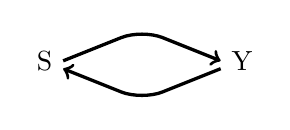
\begin{tikzpicture}
\draw[->,very thick,rounded corners=8pt] node [left] {S} (0,0) -- (1,0.4)  -- (2,0) node [right] {Y} ;
\draw[<-,very thick,rounded corners=8pt] (0,-.1) -- (1,-0.5)  -- (2,-.1)  ;	
\end{tikzpicture}		
\end{center}

We are interested in estimating 
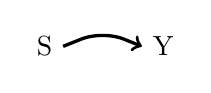
\begin{tikzpicture}[scale=0.5]
\draw[->,very thick,rounded corners=8pt] node [left] {S} (0,0) -- (1,0.4)  -- (2,0) node [right] {Y} ;
\end{tikzpicture} and not
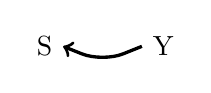
\begin{tikzpicture}[scale=0.5]
\draw[<-,very thick,rounded corners=8pt] node [left] {S} (0,0) -- (1,-0.4)  -- (2,0) node [right] {Y} ;	
\end{tikzpicture}\medskip\pause


\textbf{IV method:} Find a variable $Z$ (the instrument) that affects $Y$ \textbf{only} through $S$ and $Y_i^S\perp Z$.
\begin{center}
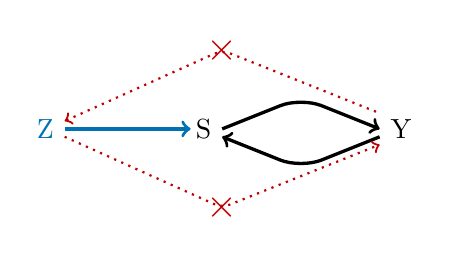
\begin{tikzpicture}
\draw[->,very thick,rounded corners=8pt] node [left] {S} (0,0) -- (1,0.4)  -- (2,0) node [right] {Y} ;
\draw[<-,very thick,rounded corners=8pt] (0,-.1) -- (1,-0.5)  -- (2,-.1)  ;	
\draw[->,blue, very thick ] (-2,0) node [left] {Z} -- (-.4,0)  ;
\color{red}
\draw[->,dotted, thick, rounded corners=3pt] (-2,-.1) -- (0,-1) node {\Large$\mathbf{\times}$} -- (2,-.2)  ;	
\draw[<-,dotted, thick, rounded corners=3pt] (-2,.1) -- (0,1) node {\Large$\mathbf{\times}$} -- (2,.2)  ;	
\end{tikzpicture}
\end{center}	
Then we can exploit $Z$ to estimate 
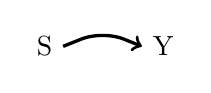
\begin{tikzpicture}[scale=0.5]
\draw[->,very thick,rounded corners=8pt] node [left] {S} (0,0) -- (1,0.4)  -- (2,0) node [right] {Y} ;
\end{tikzpicture}	
\end{frame}


\begin{frame}{Conditions for a valid instrument}
A valid instrument needs to satisfy three conditions:
\begin{enumerate}
\item \textbf{Relevance}: $Z_i$ affects the endogenous regressor $S_i$. 
\begin{center}
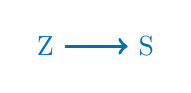
\begin{tikzpicture}[scale=0.5]
\draw[->,blue, very thick ] (-2,0) node [left] {Z} -- (-.4,0) node [right] {S} ;
\end{tikzpicture}
\end{center}
\item \textbf{Exogeneity}: $Z_i$ is as good as randomly assigned. 
\begin{center}
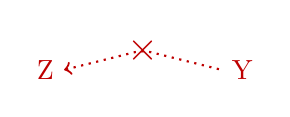
\begin{tikzpicture}[scale=0.5]
\color{red}
\draw[<-,dotted, thick, rounded corners=3pt] (-2,0) node [left] {Z} -- (0,.5) node {\Large $\mathbf{\times}$} -- (2,0) node [right] {Y} ;	
\end{tikzpicture}
\end{center}
\item \textbf{Exclusion restriction}: $Z_i$ affects $Y_i$ only through $S_i$ and not any other regressor.
\begin{center}
\begin{tikzpicture}[scale=0.5]
\color{red}
\draw[->,dotted, thick, rounded corners=3pt] (-2,0) node [left] {Z} -- (0,-.5) node {\Large $\mathbf{\times}$} -- (2,0) node [right] {Y} ;	
\end{tikzpicture}		
\end{center}
\end{enumerate}
Of these only the first condition can be tested. This is the strength of the first stage. Conditions 2 and 3 have to be argued based on knowledge from outside the data we have.
\end{frame}


\begin{frame}{Example}
Suppose the following potential outcomes model for earnings (introduced in the previous lecture):
\[Y^s_i=\alpha+\beta S_i+\eta_i,\qquad \eta_i=\gamma X_i+v_i \]
where we shall refer to $X_i$ as a vector of ``ability'' variables, and $\gamma$ is a vector of population regression coefficients so that $v_i$ and $X_i$ are uncorrelated by construction.\medskip

For now, we also assume $E[v_iS_i] = 0$ implying that the variables $X_i$ are the only reason why $\eta_i$ and $S_i$ are correlated. Hence, if $X_i$ were observable, we would estimate the following ``long'' regression using OLS:
\[Y_i =\alpha + \beta S_i + X'_i\gamma + v_i\]

\end{frame}


\begin{frame}{Example}
Now suppose that $X_i$ is unobserved. This implies our estimable equation takes the following form:
\[Y_i =\alpha+\beta S_i+\eta_i\]
where $\eta_i = X'_i\gamma
+ v_i$ is the compound error term.\medskip 

We have OVB in OLS and it doesn't work.\medskip

But if we have access to an instrument $Z_i$ that is correlated with $S_i$ and uncorrelated with $X_i$ (and thus $\eta_i$):
\[E[Z_i\eta_i]=0 \ \Rightarrow \ E[Z_i(Y_i-\alpha-\beta S_i)]=0 \ \Rightarrow \ E[Z_iY_i]=\alpha \bar{z} +\beta E[Z_i S_i] \]
using Cov$(x,y)=E[xy]-\bar{x}\bar{y}$ and $E[\eta_i]=0$ we get \[\beta=\frac{\text{Cov}(Z_i,Y_i)}{\text{Cov}(Z_i,S_i)}\]
\end{frame}



\begin{frame}{The IV solution}
	Omitted variable \qquad  \quad reverse causality \qquad
	\quad measurement error\medskip
	
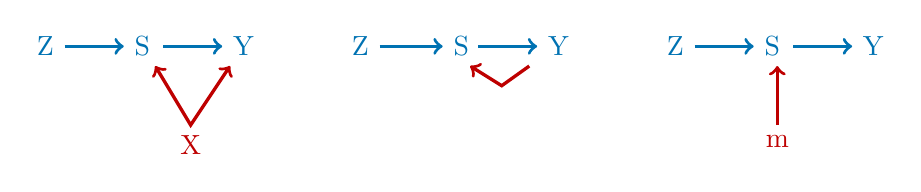
\begin{tikzpicture}[scale=0.5]
\draw[->,blue, very thick ] (-10,0) node [left] {Z} -- (-8.5,0) node [right] {S} ;
\draw[->,blue, very thick ] (-7.5,0) -- (-6,0) node [right] {Y} ;
\draw[<->,red, very thick ] (-7.7,-.5) -- (-6.8,-2) node [below] {X} --(-5.8,-.5) ;


\draw[->,blue, very thick ] (-2,0) node [left] {Z} -- (-.4,0) node [right] {S} ;
\draw[->,blue, very thick ] (.5,0) -- (2,0) node [right] {Y} ;
\draw[<-,red, very thick ] (.3,-.5) -- (1.1,-1) --(1.8,-.5) ;

\draw[->,blue, very thick ] (6,0) node [left] {Z} -- (7.5,0) node [right] {S} ;
\draw[->,blue, very thick ] (8.5,0) -- (10,0) node [right] {Y} ;
\draw[->,red, very thick ] (8.1,-2) node [below] {m} -- (8.1,-0.5) ;
\end{tikzpicture}
	
	
The IV idea is to isolate variation in $S_i$ which is unrelated to $X_i, Y_i$ or $m_i$.\medskip

The variable which does the isolating is the instrumental variable $Z_i$.\medskip

The good thing is that we just need some of the variation in $S_i$, so the requirements on the instrument seem weaker than those on the regression control $X_i$. \medskip

But IV comes with other possible complications.
\end{frame}



\begin{frame}{A bear as an IV!}
	\begin{center}
	\animategraphics[autoplay,loop,controls,width=0.6\linewidth]{12}{./Figures/IVanim/ezgif-frame-}{001}{168}
	\end{center}
\end{frame}

\subsection{IV estimation}

\begin{frame}{Three causal effects}
There are three causal effects we can think about in an IV framework:
\begin{enumerate}
\item \textbf{First stage}: The causal effect of $Z_i$ on $S_i$.
\[S_i = \pi_{10} + \pi_{11}Z_i + \zeta_{1i}\]
\item \textbf{Reduced form}: The causal effect of $Z_i$ on $Y_i$.
\[Y_i = \pi_{20} + \pi_{21}Z_i + \zeta_{2i}\]
\item \textbf{Second stage}: The causal effect of $S_i$ on $Y_i$.
\[Y_i = \alpha + \beta S_i + \eta_i \]
\end{enumerate}

The second stage is the one we are ultimately interested in.
\end{frame}

\begin{frame}{The conditions and causal effects}
\textbf{Exogeneity} and \textbf{relevance} conditions are enough for the \textbf{first stage} and \textbf{reduced form} to have a causal interpretation.\bigskip

Often, the reduced form coefficient may be interesting in its own right. For example, the instrument might be a policy variable in which case it is the policy effect.\bigskip

To get the causal effect in the \textbf{second stage}, i.e. an unbiased estimation of $\beta$, \textbf{exclusion restriction} is also necessary.\medskip

\textbf{Exclusion restriction} is often the most difficult requirement on an instrument. It is distinct from random assignment, so having experimental variation does not guarantee a valid IV interpretation of the estimates.
\end{frame}

\begin{frame}{Linking the three equations}
The coefficients in the three equations are linked. Substitute the first stage into the structural equation:
\[Y_i = \alpha + \beta S_i + \eta_i\]
\[= \alpha + \beta [\pi_{10} + \pi_{11}Z_i + \zeta_{1i} ] + \eta_i\]
\[= (\alpha + \beta \pi_{10}) + \beta \pi_{11}Z_i + (\beta\zeta_{1i} + \eta_i )\]
\[= \pi_{20} + \pi_{21}Z_i + \zeta_{2i}\]
Hence, the reduced form coefficients are:
\[\pi_{20} = \alpha + \beta \pi_{10} \qquad \pi_{21} = \beta \pi_{11}\]
\end{frame}

\begin{frame}{Indirect least squares and just-identified models}
It is straightforward to see that
\[\beta = \frac{\pi_{21}}{\pi_{11}}=\frac{\text{Cov}(Z_i,Y_i)}{\text{Cov}(Z_i,S_i)}\]
The IV estimate is equal to the ratio of the reduced form coefficient on the instrument to the first stage coefficient.\bigskip

This is called indirect least squares.
It only works when there is one endogenous regressor ($S_i$) and one instrument $Z_i$. \medskip

Such a model is called \textbf{just identified }(there is
only one single solution to get $\beta$ from the first stage and reduced form coefficients).
\end{frame}


\begin{frame}{2-Stage Least Square (2SLS)}
\[S_i = \pi_{10} + \pi_{11}Z_i + \zeta_{1i} \ \rightarrow \ \hat{S}_i = \pi_{10} + \pi_{11}Z_i \]
\[Y_i = \alpha + \beta S_i + \eta_i = \alpha + \beta \hat{S}_i + \underbrace{\beta \zeta_{1i}+\eta_i}_{\hat{\large \eta}_i}=\alpha + \beta \hat{S}_i+\hat{\eta}_i \]

Here we have Corr($S_i$,$\eta_i$)$\neq0$ but Corr($\hat{S}_i,\hat{\eta}_i$)$=0$ or $E[\hat{S}_i\hat{\eta}_i]=0$. \medskip

Thus, we can find $\beta$ by regressing $Y_i$ on $\hat{S}_i$ with OLS method.\medskip

This method is called Two-Stage Least Squares (2SLS):
\begin{enumerate}
\item First stage: regress $S_i$ on $Z_i$ and predict $\hat{S}_i$.
\item Second stage: regress $Y_i$ on $\hat{S}_i$ and find $\beta$.
\end{enumerate}
\end{frame}

\begin{frame}{Over-identified models}
Many times a single instrument is not strong enough (we'll see what that means) and we might use multiple instruments ($Z_1, Z_2,\dots$) for a single endogenous regressor ($S_i$).\medskip

Such a model is called \textbf{over-identified.}

\[S_i = \pi_{10} + \pi_{11}Z_{1i} + \pi_{12}Z_{2i} + \zeta_{1i}\]
\[Y_i = \pi_{20} + \pi_{21}Z_{1i} + \pi_{22}Z_{2i} + \zeta_{2i} \]
There is no unique way to get $\beta$ from $\pi_{11}, \pi_{12}, \pi_{21}$, and $\pi_{22}$. \medskip

Indeed, we now have one unknown parameter ($\beta$), but two equations which are called ``moment conditions'': \[E[Z_{1i}\eta_i]=0 ,\quad E[Z_{2i}\eta_i]=0\]


% 3SLS is a method for Simultaneous equations not IVs with one equation.

\end{frame}

\begin{frame}{2SLS with multiple instruments}
With multiple instrument, we cannot use indirect least square, but 2SLS still works:
\begin{enumerate}
\item First stage: regress $S_i$ on both $Z_{1i}$ and $Z_{2i}$ and predict $\hat{S}_i$
\[S_i = \pi_{10} + \pi_{11}Z_{1i} + \pi_{12}Z_{2i} + \zeta_{1i}\ \Rightarrow \ \hat{S}_i = \pi_{10} + \pi_{11}Z_{1i} + \pi_{12}Z_{2i}\] 
\item Second stage: regress $Y_i$ on $\hat{S}_i$ and find $\beta$: \[Y_i = \alpha + \beta \hat{S}_i + \eta_i\]
\end{enumerate}

But how 2SLS estimates one parameter $\beta$ using multiple equations $E[Z_{1i}\eta_i]=0 ,\ E[Z_{2i}\eta_i]=0$? 
\end{frame}

\begin{frame}{2SLS as a GMM estimation}
Two stage least squares (2SLS) is a special case of GMM estimator for the homoskedastic moment condition ($\Omega=\sigma^2I_n$).\bigskip

Indeed the 2SLS estimation is the previous example with $Z_1$ and $Z_2$ as instrument can be written as

\[ \min_{\alpha, \beta} E[(Z_{1i}\eta_i,\ Z_{2i}\eta_i)].E\Big[\Big(\begin{array}{c}
Z_{1i}\eta_i\\ Z_{2i}\eta_i
\end{array}\Big)\Big] \] 

If you solve this analytically (using matrix notation), you get same estimation of $\alpha , \beta$ as the previous example.\bigskip

In 2SLS estimation of over-identified models, we implicitly assume that the instrument are equally important and uncorrelated to each other.
\end{frame}


\begin{frame}{STATA commands for IV}

Useful STATA commands
\begin{itemize}
\item 2SLS: \texttt{ivreg2 y (s = z) } 
\item Two-step GMM: \texttt{ivreg2 y (s = z),  gmm2s} 
\item Continuously-updated GMM: \texttt{ivreg2 y (s = z),  cue} 
\end{itemize}

\end{frame}


%\begin{frame}{The Wald estimator}
%Provides a good intuition that why exclusion restriction is important.\medskip
%
%Assume $z$ is a binary (0-1) satisfying the two conditions, then
%\[E[y_i|z_i]= \alpha+\beta E[x_i|z_i] \ \Rightarrow \ \beta=\frac{E[y_i|z_i=1]-E[y_i|z_i=0]}{E[x_i|z_i=1]-E[x_i|z_i=0]} \]
%If the exclusion restriction does not hold $E[z_iA_i]\neq0$:
%\[E[y_i|z_i]= \alpha+\beta E[x_i|z_i]+\gamma E[A_i|z_i] \] \[\Rightarrow \ \beta=\frac{E[y_i|z_i=1]-E[y_i|z_i=0]}{E[x_i|z_i=1]-E[x_i|z_i=0]}{\color{red} -\gamma\frac{E[A_i|z_i=1]-E[A_i|z_i=0]}{E[x_i|z_i=1]-E[x_i|z_i=0]}} \]
%
%The \textit{only} reason for any relation between the  dependent variable $y$ and the instrument $z$ is the effect of instrument on endogenous variable $x$.
%\end{frame}

\subsection{Weak instrument}

\begin{frame}{Weak instruments}
\[\beta^{IV}=\frac{Cov(Y,Z)}{Cov(S,Z)}=\beta+\frac{Cov(\eta,Z)}{Cov(S,Z)} \]
A good IV satisfies $Cov(\eta,Z)=0, \ Cov(S,Z)\neq 0 \Rightarrow \beta^{IV}=\beta$\medskip

If the first stage is weak, $Cov(S,Z)$ is small and we have weak instruments problem.\medskip

It can be that $Cov(S,Z)$ is truely zero but in a finite sample the estimated $Cov(S,Z)$  will not be exactly zero and we get a biased estimate. \medskip

The 2SLS estimator with weak instruments is biased in small samples.\medskip

Any inconsistency from a small violation of the exclusion restriction gets magnified by weak instruments.\medskip


The bias will tend to be worse in overidentified models with many instruments compared to endogenous regressors.
\end{frame}

\begin{frame}{Testing relevance of the instrument}
F-test for relevance condition tests the null that the coefficients of all instruments are jointly zero. 
\[S_i = \pi_{10} + \pi_{11}Z_{1i} + \pi_{12}Z_{2i} + X'\gamma + \zeta_{1i}\quad H_0: \pi_{11}=\pi_{12}=0 \]


Staiger and Stock (1997) show that we need the following for F-test in the first stage 

\begin{itemize}
\item Maximal bias in IV be no more than 10\% of OLS we need $F>10$.
\item Maximal bias in IV be no more than 20\% of OLS, we need $F>6.5$.
\end{itemize}

F-statistic above 10 to 20 are considered relatively safe, lower
F-statistics alarm the danger of weak instrument.
\end{frame}

\begin{frame}{How to cope with weak instrument}
With weak instruments
\begin{itemize}
\item 2SLS is biased towards OLS.
\item Estimated standard errors of 2SLS estimators may be too small.
\item Adding more weak instruments will increase the bias of 2SLS and the first stage F-statistic goes towards 0.
\item Weak instrument bias is less of a problem in just identified models 
\end{itemize}\medskip

We have the following options:
\begin{itemize}
\item Use a just identified model with the strongest IV.
\item Use LIML instead of 2SLS which have better small sample
properties with weak instruments and for overidentified models. \texttt{ivreg2 y (s = z1 z2) x , liml}
\item Find stronger instruments.
\end{itemize} 

\end{frame}

\subsection{IV examples}

\begin{frame}{Finding an instrument}
We should build natural or quasi experiments using law changes / events / randomness that directly affects a variable and through which other outcomes.
\begin{itemize}
\item Theory combined with clever data collection \begin{itemize}
\item distance from job training center varies the cost of participation in training, and we're interested in the effect of training on wages
\end{itemize}\medskip

\item Exogenous variation in policies or program implementation, over time or across space \begin{itemize}
\item Vietnam draft lottery, interested in the effect of military service on wages
\end{itemize}\medskip

\item Nature \begin{itemize}
\item stormy weather varies the supply of fish, which allows us to learn how price sensitive demand for fish sticks really is
\end{itemize}
%\item Roll Your Own (Example: an experiment, or randomized encouragement to take up treatment if experiment is infeasible/unethical) LATE estimation
\end{itemize}
\end{frame}

\begin{frame}{Angrist and Krueger (1991)}
To estimate the effect of schooling on wage, Angrist and Krueger (1991) used quarter of birth as an instrumental variable for schooling.\bigskip

In the US children are required to go to school in calendar year they turn 6 and they could drop out of school once they turned 16.\medskip

Children have different ages when they start school and thus different lengths of schooling at the time they turn 16 when they can potentially drop out.

\begin{figure}
\centering
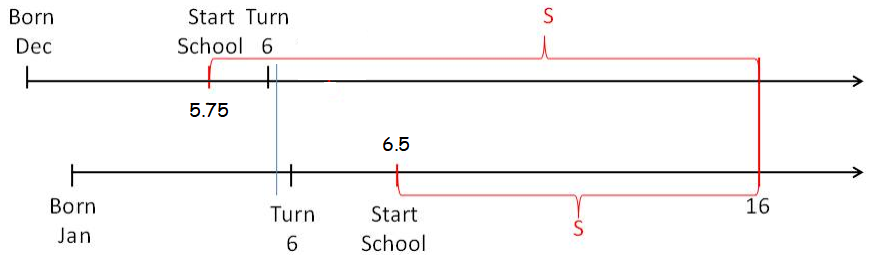
\includegraphics[width=.8\linewidth]{./Figures/angristkrueger91}
\end{figure}
\end{frame}

\begin{frame}{Checking three conditions for IV}
\textbf{Relevance:} Do birthdays affects schooling?\pause
\begin{itemize}
\item Check the first stage and its F-statistic.
\end{itemize}\bigskip

\textbf{Exogeneity:} Are birthdays random with respect to the
counterfactual earnings for different schooling levels?\pause
\begin{itemize}
\item It seems so.
\end{itemize}\bigskip

\textbf{Exclusion restriction:} Do birthdays satisfies the exclusion restriction, or could birthdays be correlated with earnings for other reasons than their effect on schooling?\pause
\begin{itemize}
\item Some sort of family background is associated with the quarter of birth.
\end{itemize}
\end{frame}




\begin{frame}{Angrist and Krueger (1991) -- First stage}
%\[S_i = X'\Pi_{10} + \pi_{11}Z_i + \zeta_{1i}\]
People born in earlier seasons of the year have lower schooling.
\begin{figure}
\centering
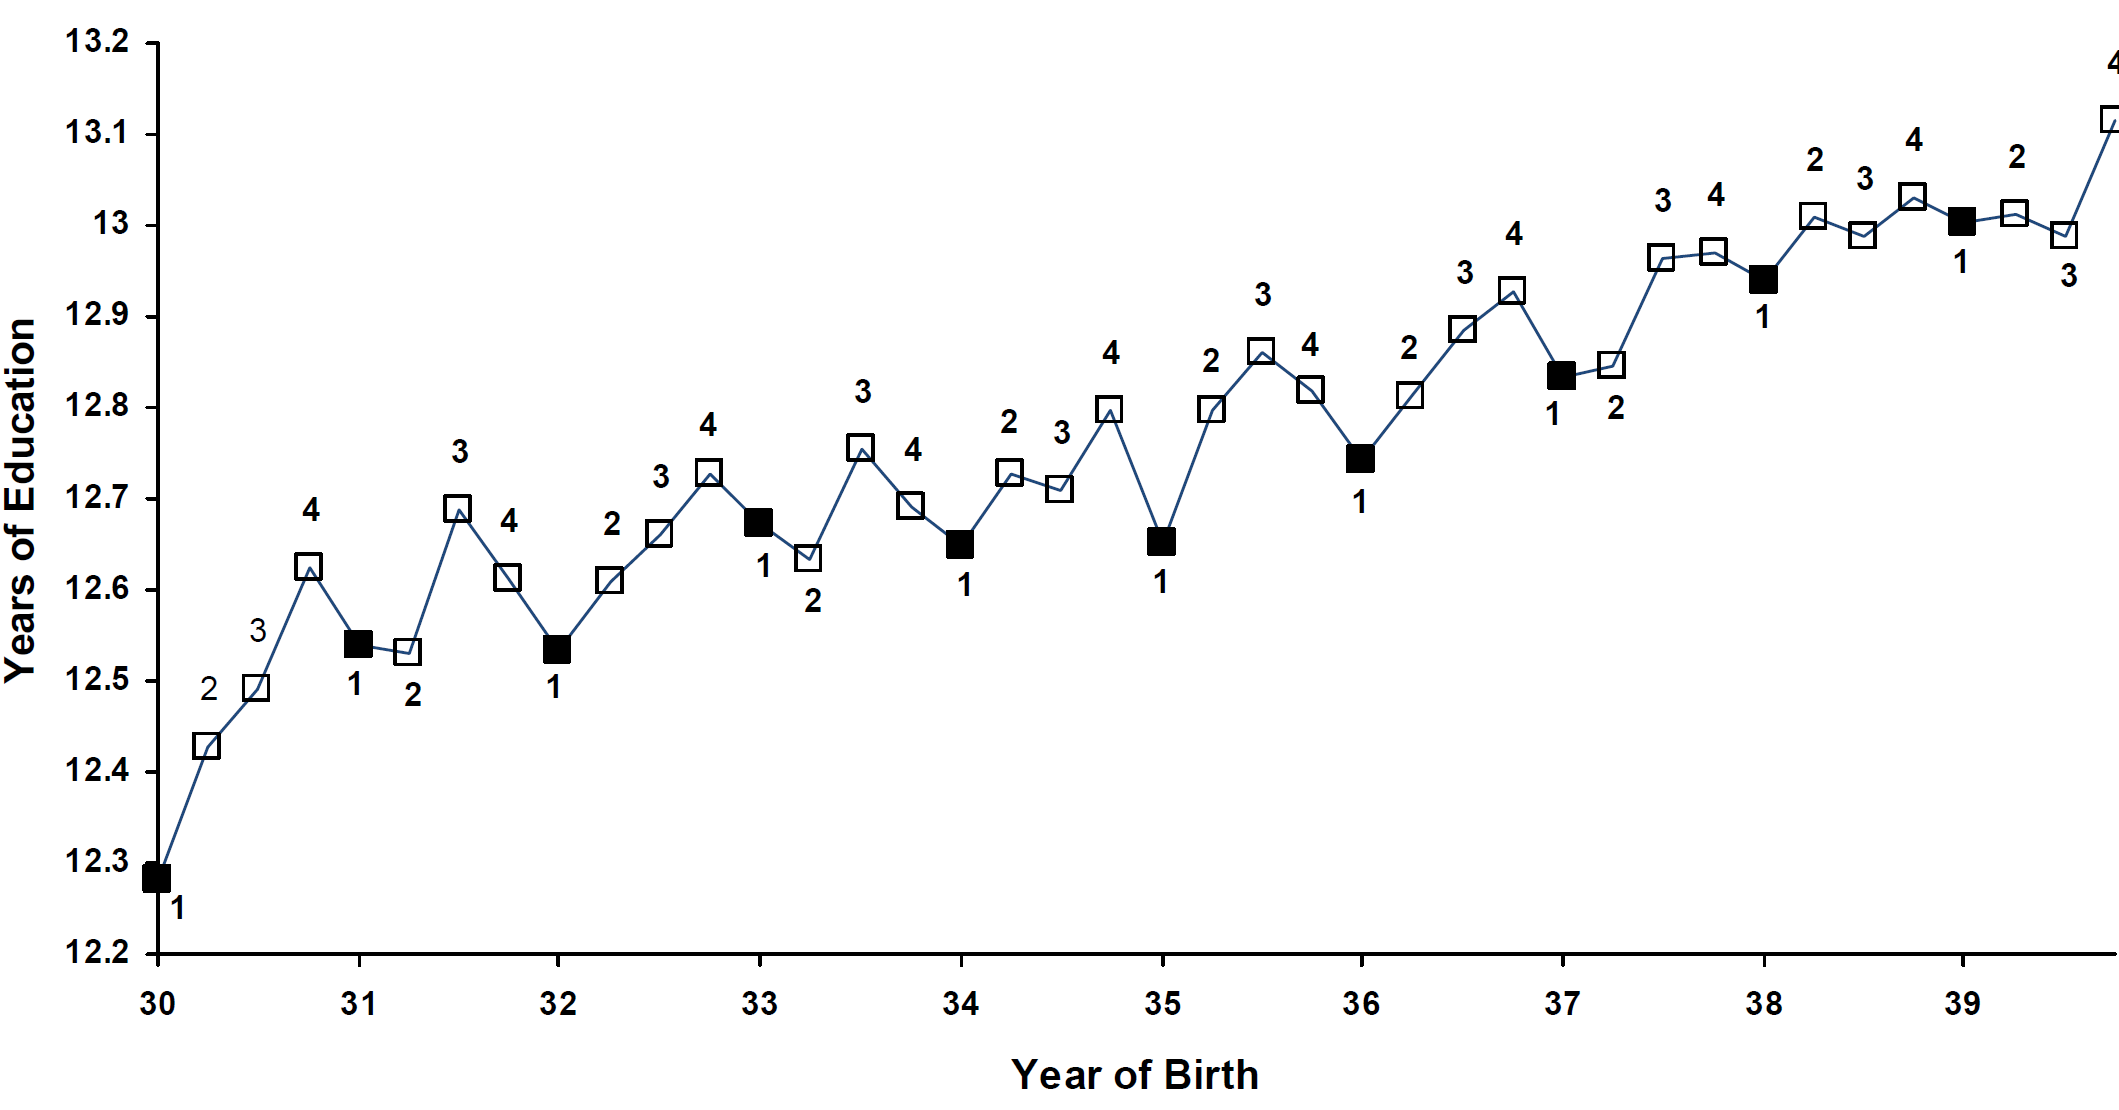
\includegraphics[width=.8\linewidth]{./Figures/angristkrueger2}
\end{figure}

\end{frame}

\begin{frame}{Angrist and Krueger (1991) -- Reduced form}
%Difference in earning and quarter of birth. 
\begin{figure}
\centering
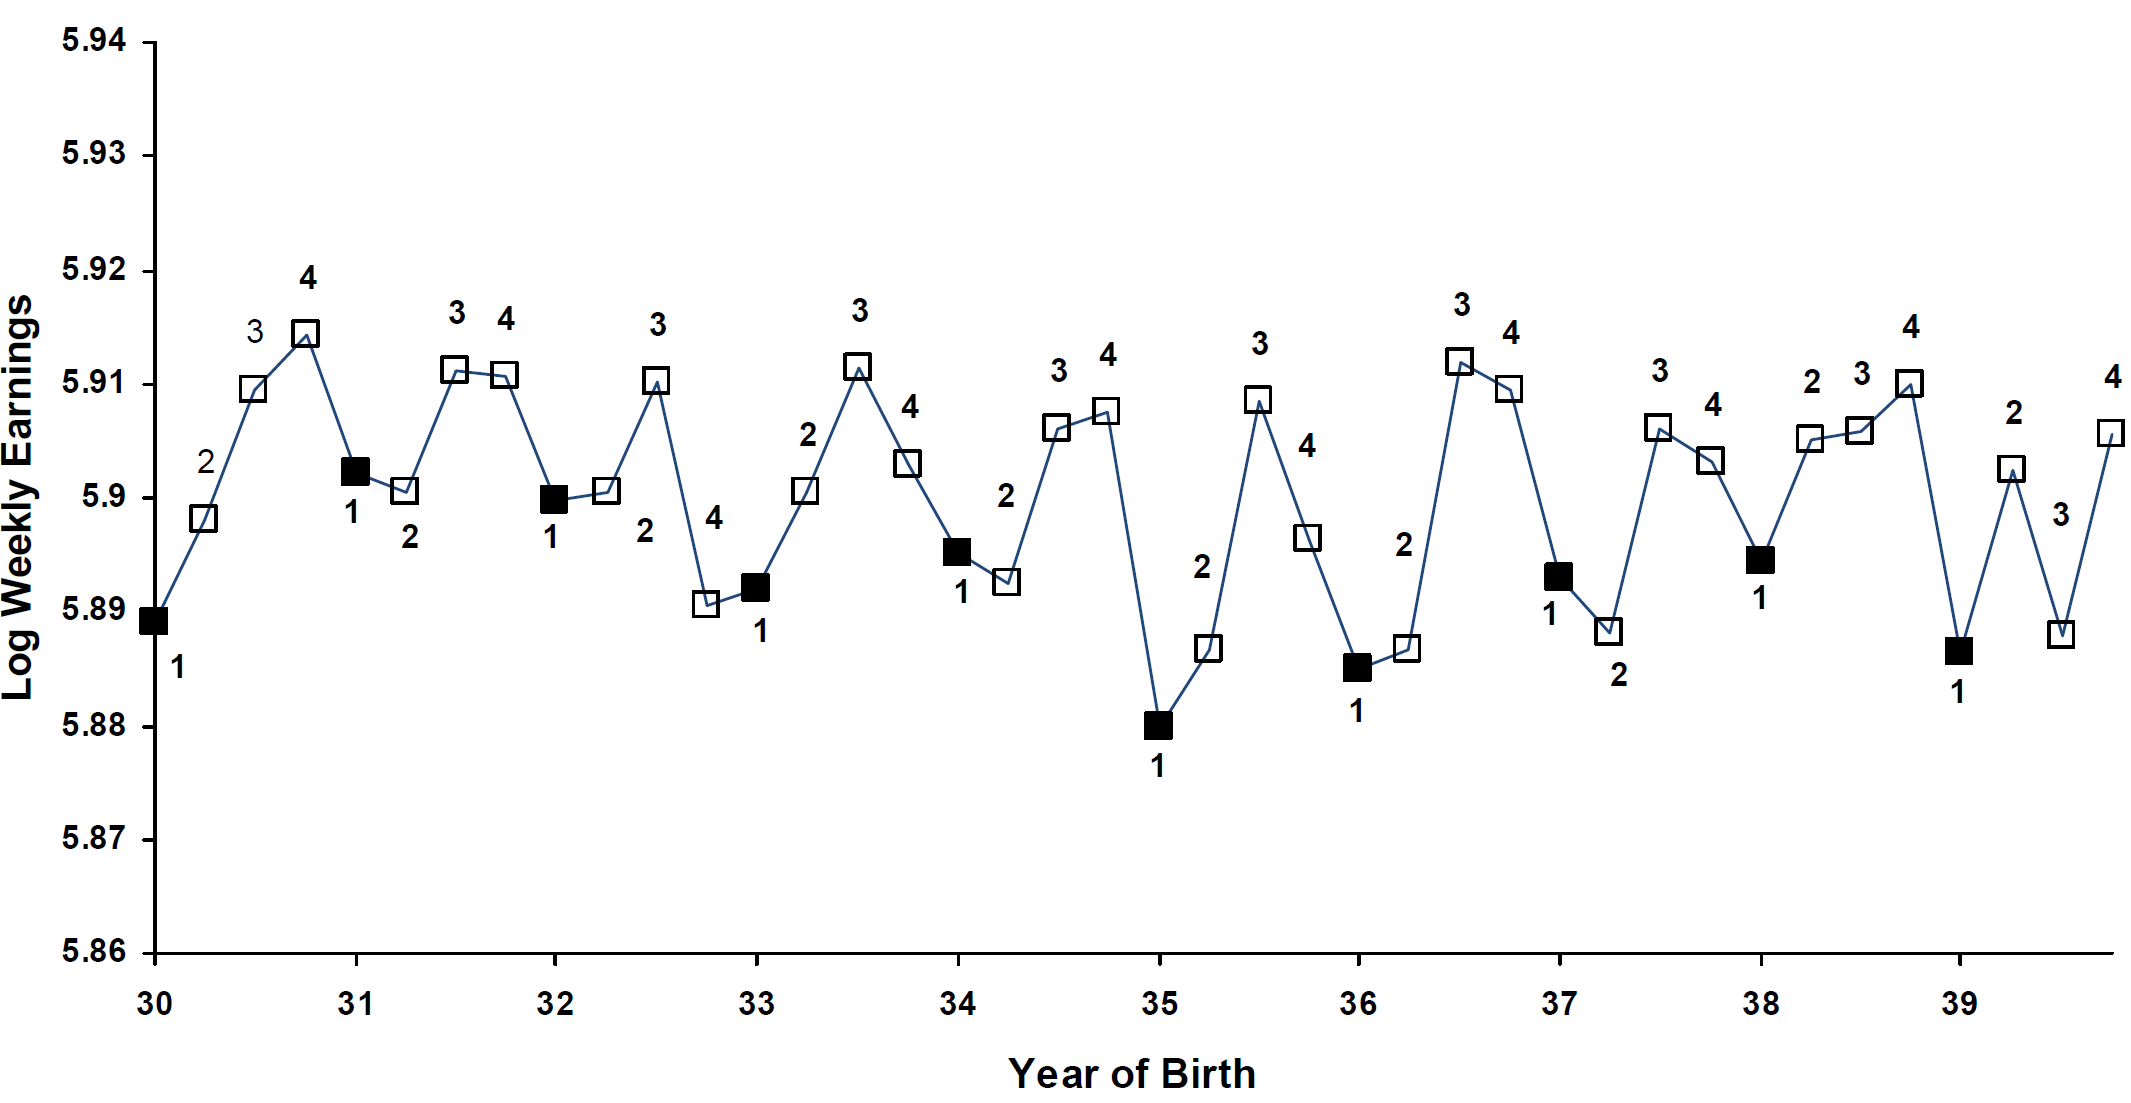
\includegraphics[width=.8\linewidth]{./Figures/angristkrueger3}
\end{figure}
Do differences in schooling due to different quarter of birth leads to different earnings?
\end{frame}

\begin{frame}{Angrist and Krueger (1991) -- Regression setup}
The consider three dummies for each quarter of birth as instrumental variables.
\[ S_i = \pi_{10} + \pi_{11}Z_{1i} + \pi_{12}Z_{2i} + \pi_{13}Z_{3i}+ X'_i\Pi_{10} + \zeta_{1i}\]
$Z_{Ji}$ is 1 if individual $i$ was born in quarter $J$ otherwise is zero. $X$ is a vector of control variables.\bigskip

The second stage uses the fitted values are from the first stage.
\[Y_i = \alpha + \beta \hat{S}_i+ X'_i\gamma + \eta_{i} \]
\end{frame}

\begin{frame}{First stage estimation}
\begin{figure}
\centering
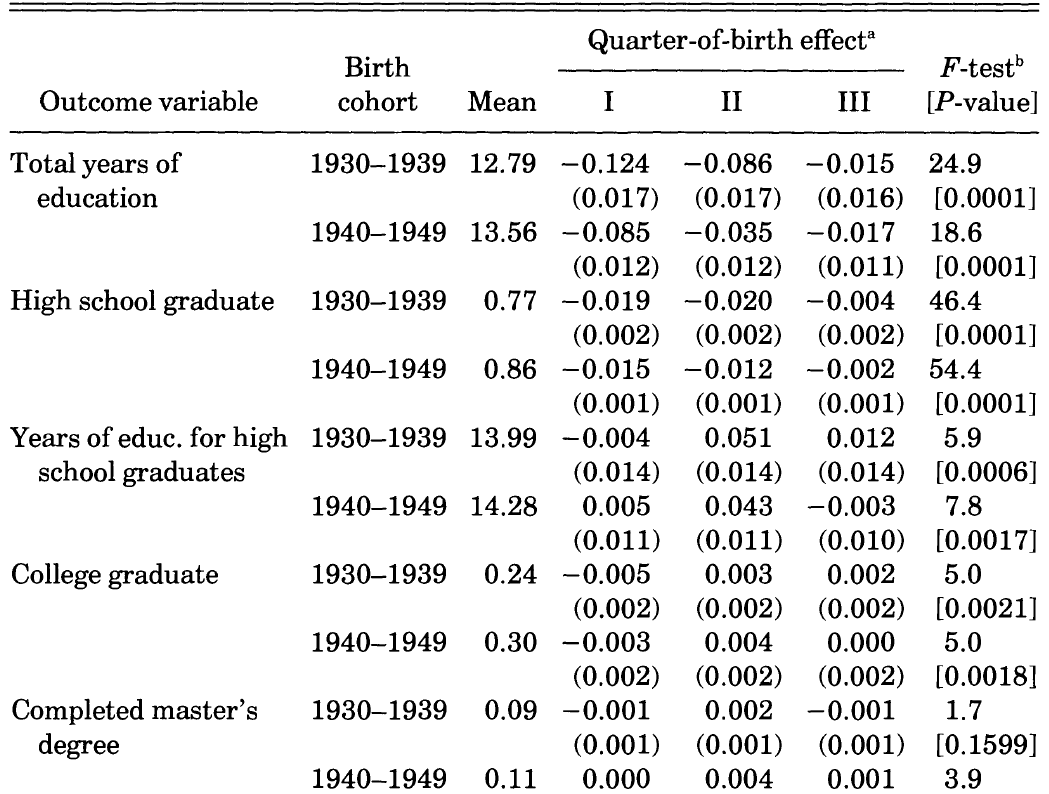
\includegraphics[width=0.5\linewidth]{./Figures/angristkrueger5}
\end{figure}
\footnotesize Quarter of birth is a strong predictor of total years of education but doesn't  affect the probability of graduating from college/ master degree.
\end{frame}

\begin{frame}{Second stage estimation}
\begin{figure}
\centering
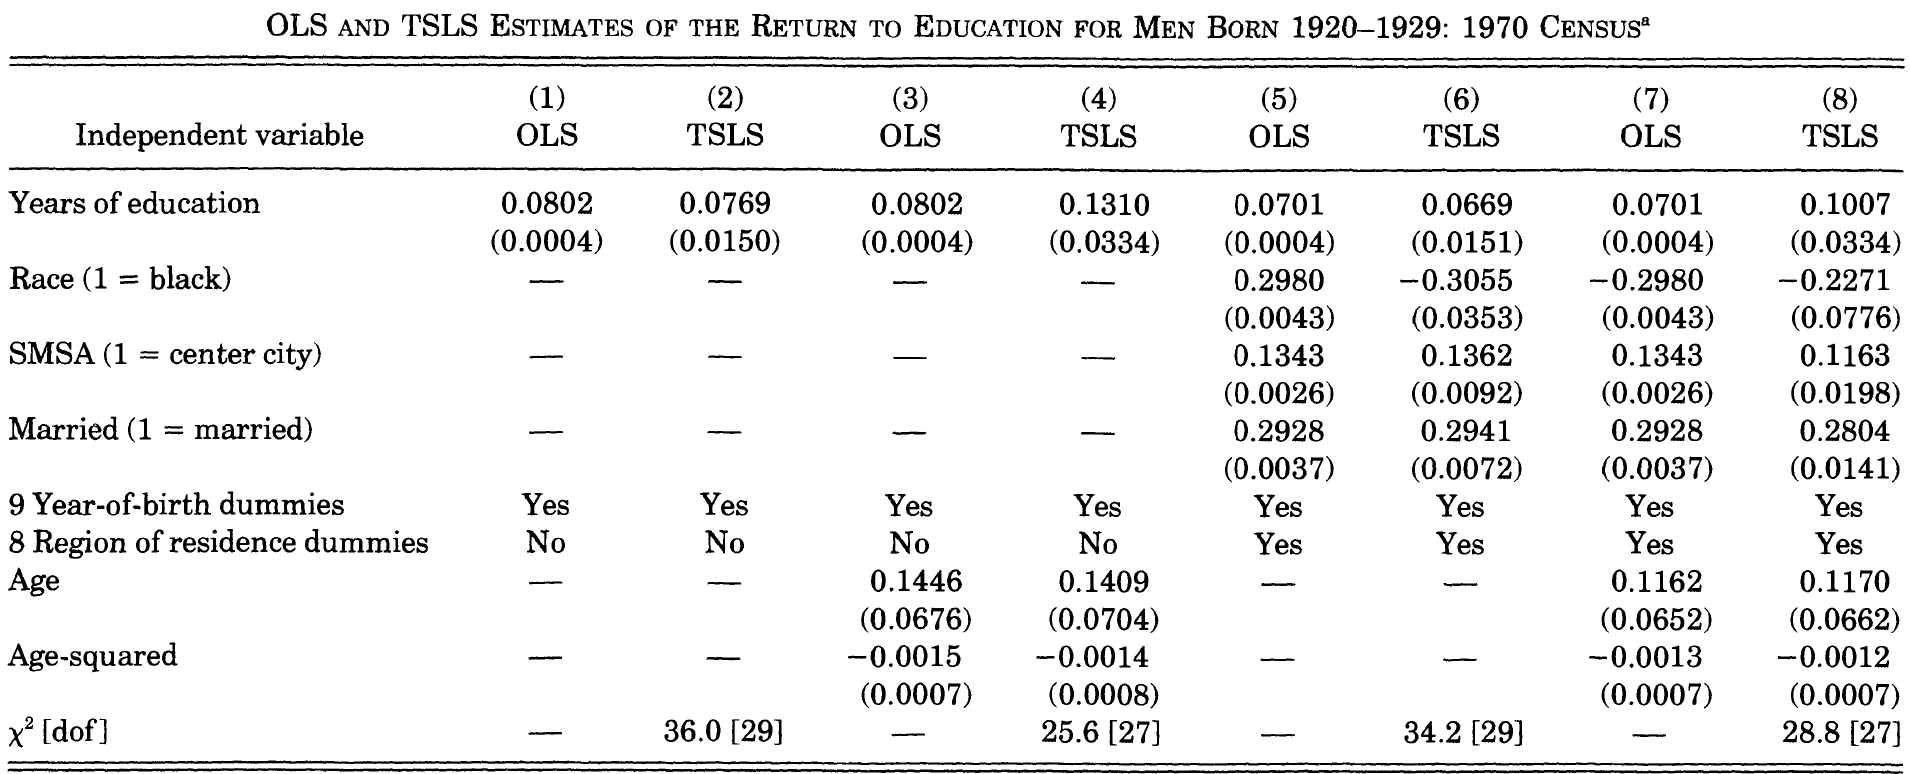
\includegraphics[width=0.95\linewidth]{./Figures/angristkrueger4_}
\end{figure}
% X^2 statistic is Sargan test of overidentifing restrictions
\end{frame}

\begin{frame}{Weak instrument problem in Angrist \& Krueger (1991)}
Angrist and Krueger use birth time and place as IV in 3 set-ups:
\begin{itemize}
\item quarter of birth dummies = 3 instruments.
\item quarter  + quarter $\times$ year dummies = 30
instruments.
\item quarter + quarter $\times$ year + quarter $\times$ state = 180 instruments.
\end{itemize}\bigskip

Bound, Jaeger, and Baker (1995) highlight weak instrument problem here and argue that the quarter of birth instruments explain only a tiny proportion of the variation in schooling leading to two problems:
\begin{itemize}
\item The 2SLS estimator with weak instruments is biased in small samples. 
\item Adding more weak instruments will increase the bias of 2SLS. The first stage
F-statistic goes towards 0 and the bias increases.
\end{itemize}\end{frame}

\begin{frame}{Bound, Jaeger, and Baker (1995)}
\begin{figure}
\centering
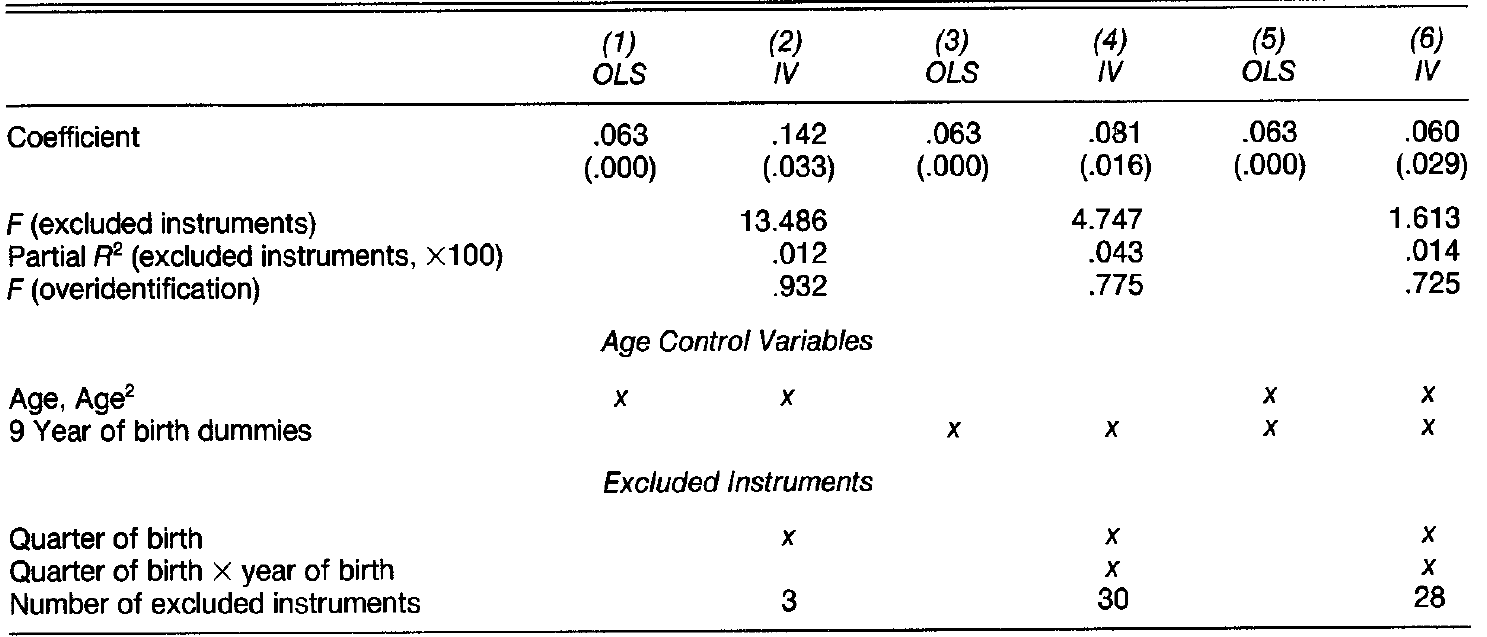
\includegraphics[width=.9\linewidth]{./Figures/boundJaeger}
\end{figure}
Adding more weak instruments reduced the first stage F-statistic and moves the coefficient towards the OLS coefficient.
\end{frame}

\begin{frame}{Example: Angrist (1990)}
The effects of military service on earnings.\medskip

Angrist (1990) uses the Vietnam draft lottery as in IV for military
service.\medskip

In the 1960s and early 1970s, young American men were drafted for
military service to serve in Vietnam.
Concerns about the fairness of the conscription policy lead to the
introduction of a draft lottery in 1970.\medskip

From 1970 to 1972 random sequence numbers were assigned to each
birth date in cohorts of 19-year-olds.\medskip

Men with lottery numbers below a cutoff were drafted while men with
numbers above the cutoff could not be drafted.\medskip


However, the draft did not perfectly determinate military service
\begin{itemize}
\item Many draft-eligible men were exempted for health reasons.
\item Also some exempted men volunteered for service.
\end{itemize}

\end{frame}

\begin{frame}{Angrist (1990)}
First stage results:
\begin{itemize}
\item Having a low lottery number (being eligible for the draft) increases veteran status by about 16 percentage points (the mean of veteran status is about 27 percent).
\end{itemize}\medskip

Second stage results:
\begin{itemize}
\item Serving in the army lowers earnings by between \$2,050 and \$2,741
per year.
\end{itemize}
\end{frame}

\begin{frame}{The effects of police officers on crime}
Endogeneity:  The number of police officers a community hires is influenced by the
community's crime rate\medskip

Levitt (1997) proposes local election as instruments for the number of police officers, on the idea that changes in the number of officers would be correlated with mayors and governors running for re-election.\medskip

McCrary (2002) showed that a programming error in Levitt's (1997) led to an IV estimate
that was too large and erroneously significant.\medskip

Levitt (2002) reassesses the effect by using the number of firefighters in a city as an instrument for the number of police.

%Factors such as the power of public sector unions, citizen tastes for government services, affirmative action initiatives, or a mayor's desire to provide spoils might all be expected to jointly influence the number of firefighters and police. Empirically, changes in the number of police officers and firefighters within a city are highly correlated over time. 
\end{frame}

\begin{frame}{Other examples}

Natural experiments:
\begin{itemize}
\item Financial development and Growth: Legal origin as an instrument for financial development (La Porta, Shleifer, Vishny, 1998 QJE)

\item Access to bank on poverty: A policy change to increase rural branches in India (Burgess and Pande, 2005 AER)
\end{itemize}\medskip
Using household characteristics as  instruments:
\begin{itemize}
\item Accept lower wages in exchange for health benefits? Olson (2002 JLE) estimate this for women using husband's union status, husband's firm size, and husband's health coverage through his job. 

\end{itemize}\end{frame}

\begin{frame}{Some advice for doing IV}
Good IVs come from institutional knowledge and your idea about the process of determining the endogenous variable. With this knowledge,
you should convince the readers that your instrument is exogenous and affects outcome only thorough the endogenous variable. \medskip

In other words, there is no credible statistical test for showing exogeneity and exclusion restriction and you should make your arguments based on theory or some facts and background information.\medskip

For the relevance condition, report the first stage and check the sign of instrument. Also check the F-statistics and whether it is above 10. \medskip 

If you have many IVs pick your best instrument and report the justidentified model. In overidentified model compare 2SLS with LIML.\medskip

Report the reduced-form regression (using OLS). If you don't see an effect in reduced-form while your instrument is good, your causal effect of interest is probably insignificant. 
\end{frame}


%\begin{frame}{References:}
%\bibliographystyle{apalike}
%\small
%\bibliography{references}
%\end{frame}

\end{document}
